\section{Antiferromagnetic Heisenberg Chain,}
\subsection{Review of the Heisenberg Chain}
Recall the Heisenberg spin chain Hamiltonian:
\begin{equation}\label{eq:Heisenbergchain}
    \hat{H} = -J\sum_m\left(\hat{S}^z_m\hat{S}^z_{m+1} + \frac{1}{2}\left(\hat{S}^+_m\hat{S}^-_{m+1} + \hat{S}^-_m \hat{S}^+_{m+1}\right)\right)
\end{equation}
and after the Holstein-Primakoff transformation, this became:
\begin{equation}
    \hat{H} = -JNS^2 + JS\sum_{m}\left(\hat{a}^\dag_m\hat{a}_m + \hat{a}^\dag_{m+1}\hat{a}_{m+1} - \hat{a}^\dag_m\hat{a}_{m+1} - \hat{a}^\dag_{m+1}\hat{a}_m\right) + O(S^0)
\end{equation}
Note to get here we first did an exact transformation into bosonic operators, then expanded this transformation in a Taylor series to obtain a Hamiltonian quadratic in $\hat{a}/\hat{a}^\dag$. This can be turned into a field theory; loosely, we can replace the $a$s by field operators:
\begin{equation}
    \hat{a}_m \to \hat{\phi}(x), \quad \hat{a}^\dag_m \to \hat{\phi}^\dag(x)
\end{equation}
Further, we can consider:
\begin{equation}
    \hat{a}_{m+1} \approx \hat{a}_m + \dpd{}{x}\hat{a}_m
\end{equation}
which can give us $\nabla \hat{\phi}$ terms. We also have the promotion of the commutators to the continuum:
\begin{equation}
    [\hat{a}_m, \hat{a}^\dag_{m'}] = \delta_{mm'} \to [\hat{\phi}(x), \hat{\phi}^\dag(x')] = \delta(x - x')a
\end{equation}
Note that this would give us a free field theory (as the bosonic operator terms are all quadratic).

\subsection{Antiferromagnetic Case}
Formally, we change the sign of $J$ in Eq. \eqref{eq:Heisenbergchain} so that it is now $J < 0$. Now, we guess our ground state to be alternating between spin up/down, with spins on the A sublattice being up and those on the B sublattice being down:

\begin{figure}[htbp]
    \centering
    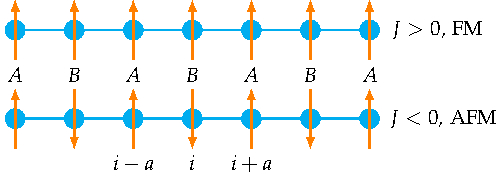
\includegraphics[scale=0.5]{Lectures/Figures/FMAFMHeisenbergchain.pdf}
    \caption{Cartoon picture of FM and AFM Heisenberg chain. $J > 0$ (ferromagnet) encourages the spins to align, while $J < 0$ (antiferromagnet) encourages the spins to anti-align. Our guess for the ground state in this case is to bipartition the chain into two sublattices, $A, B$ for spins pointing up and down. We do note that this is an ansatz/guess for the ground state, and is not an exact eigenstate of the quantum Hamiltonian.}
    \label{fig:FMAFMHeisenbergchain}
\end{figure}
So, let us consider applying a $\pi$ rotation on the $B$ sublattice of spins, i.e. taking:
\begin{equation}
    S^z_B \to -S^z_B, \quad S^y_B \to -S^y_B, \quad S^x_B \to S^x_B
\end{equation}
So the Hamiltonian becomes:
\begin{equation}\label{eq:AFMHeisenbergchain}
    \hat{H} = -\abs{J}\sum_m\left(\hat{S}^z_m\hat{S}^z_{m+1} - \frac{1}{2}\left(\hat{S}^+_m\hat{S}^+_{m+1} + \hat{S}^-_m \hat{S}^-_{m+1}\right)\right)
\end{equation}
or with the H.P. transformation:
\begin{equation}\label{eq:AFMHeisenbergchainHP}
    \hat{H} = -\abs{J}NS^2 + \abs{J}S\sum_{m}\left(\hat{a}^\dag_m\hat{a}_m + \hat{a}^\dag_{m+1}\hat{a}_{m+1} - \hat{a}_m\hat{a}_{m+1} - \hat{a}^\dag_{m+1}\hat{a}^\dag_m\right) + O(S^0)
\end{equation}
If we diagonalize this (which we can always do - it is a quadratic form!) we obtain:
\begin{equation}
    \hat{H} = -N\abs{J}S(S+1) + \abs{J}S\sum_k \m{\hat{a}^\dag_k & \hat{a}_k}\m{1 & \cos k \\ \cos k & 1} \m{\hat{a}_{-k} \\ \hat{a}^\dag_{-k}}
\end{equation}
where:
\begin{equation}
    \hat{a}_k = \sum_m e^{ikm}\hat{a}_m
\end{equation}
Now doing a Bogoulibov transformation:
\begin{equation}
    \m{\hat{\alpha}_k \\ \hat{\alpha}^\dag_{-k}} = \m{\cosh \theta_k & -\sinh \theta_k \\ -\sinh\theta_k & \cosh\theta_k}\m{\hat{a}_k \\ \hat{a}^\dag_{-k}}
\end{equation}
with $\tanh 2\theta_k = \cos k$. With this rotation, $\hat{H}$ becomes:
\begin{equation}
    \hat{H} = -N\abs{J}S^2 + 2\abs{J}S\sum_k(\sin k)\hat{\alpha}^\dag_k \hat{\alpha}_k
\end{equation}
Which gives us the spectrum - it is linear! We can think of these eigenstates as linear superpositions of spin waves in the original basis.

Unfortunately, we aren't quite done. These operators are not conserved. Because the ground state is defined by $\hat{\alpha}_k\ket{0} = 0$, but $\hat{\alpha}_k$ is a combination of $a^\dag/a$s and so can create excitations.

Let us look at the magnetization of the ground state:
\begin{equation}
    M = \bra{0} \frac{1}{N}\sum_i \hat{S}^z_i\ket{0} = S - \frac{1}{N}\sum_i \bra{0}a^\dag a \ket{0} = S - \frac{1}{N}\sum_k \sinh^2\theta_k
\end{equation}
I.e. we see it is nonzero! These are quantum fluctuations on top of the classical ground state. Looking at the integral form for this, we have:
\begin{equation}
    M = S - \int_0^{1/a}dk \frac{1}{k} k^{d-1}
\end{equation}
which diverges at $k = 0$ for $d = 1$. An important note to make; fluctuations, even quantum ones, can destroy phase transitions! E.g. the 1D classical Heisenberg model orders, the quantum one does not. But of course when we look at thermal fluctuations thing disorder even more.

The fact that $M$ diverges in 1D tells us that the approximation (i.e doing the sublattice divisions...) we made at the beginning was incorrect. This sublattice division is incorrect as there is no local $SU(2)$ symmetry (only a global one). This might have been okay if I was just asking about long range order. If $M$ turned out to be finite, we would still have a magnet... but here that is not the case.

\subsection{Phase Transitions in the Classical Magnet}
We consider a classical magnet (i.e. a lattice of classical spins), subject to two parameters, an external magnetic field $h$ and a temperature $T$. We consider the magnetization $m(T)$, which is something we may measure in a lab:
\begin{equation}
    m(T) = \frac{1}{V}\lim_{h \to 0}M(h, t)
\end{equation}
where:
\begin{equation}
    M(h, T) = \frac{1}{N}\sum_i S_i
\end{equation}
is a quantity that depends on the external field and temperature.

We have the scaling of the magnetization:
\begin{equation}
    m(T, h=0) = \begin{cases}
        0 & t > 0
        \\ \abs{t}^\beta & t < 0
    \end{cases}
\end{equation}
with $t = \frac{T_c - T}{T}$. We can also consider the scaling of $m$ w.r.t. $h$ at the critical temperature:
\begin{equation}
    m(T = T_c, h) \propto h^{1/\delta}.
\end{equation}
The $\beta, \delta$ appearing above are the critical exponents that quantify the phase transition.

We may also consider the measurement of a response function, i.e. the response of the system to some perturbation that we put in. An example is the magnetic susceptibility $\chi$:
\begin{equation}
    \chi(T, h =0) = \dpd{m}{h}
\end{equation}
or the specific heat:
\begin{equation}
    C = \left.\dod{E}{T}\right|_T \propto c \abs{t}^{-\alpha_\pm}
\end{equation}

\begin{figure}
    \centering
    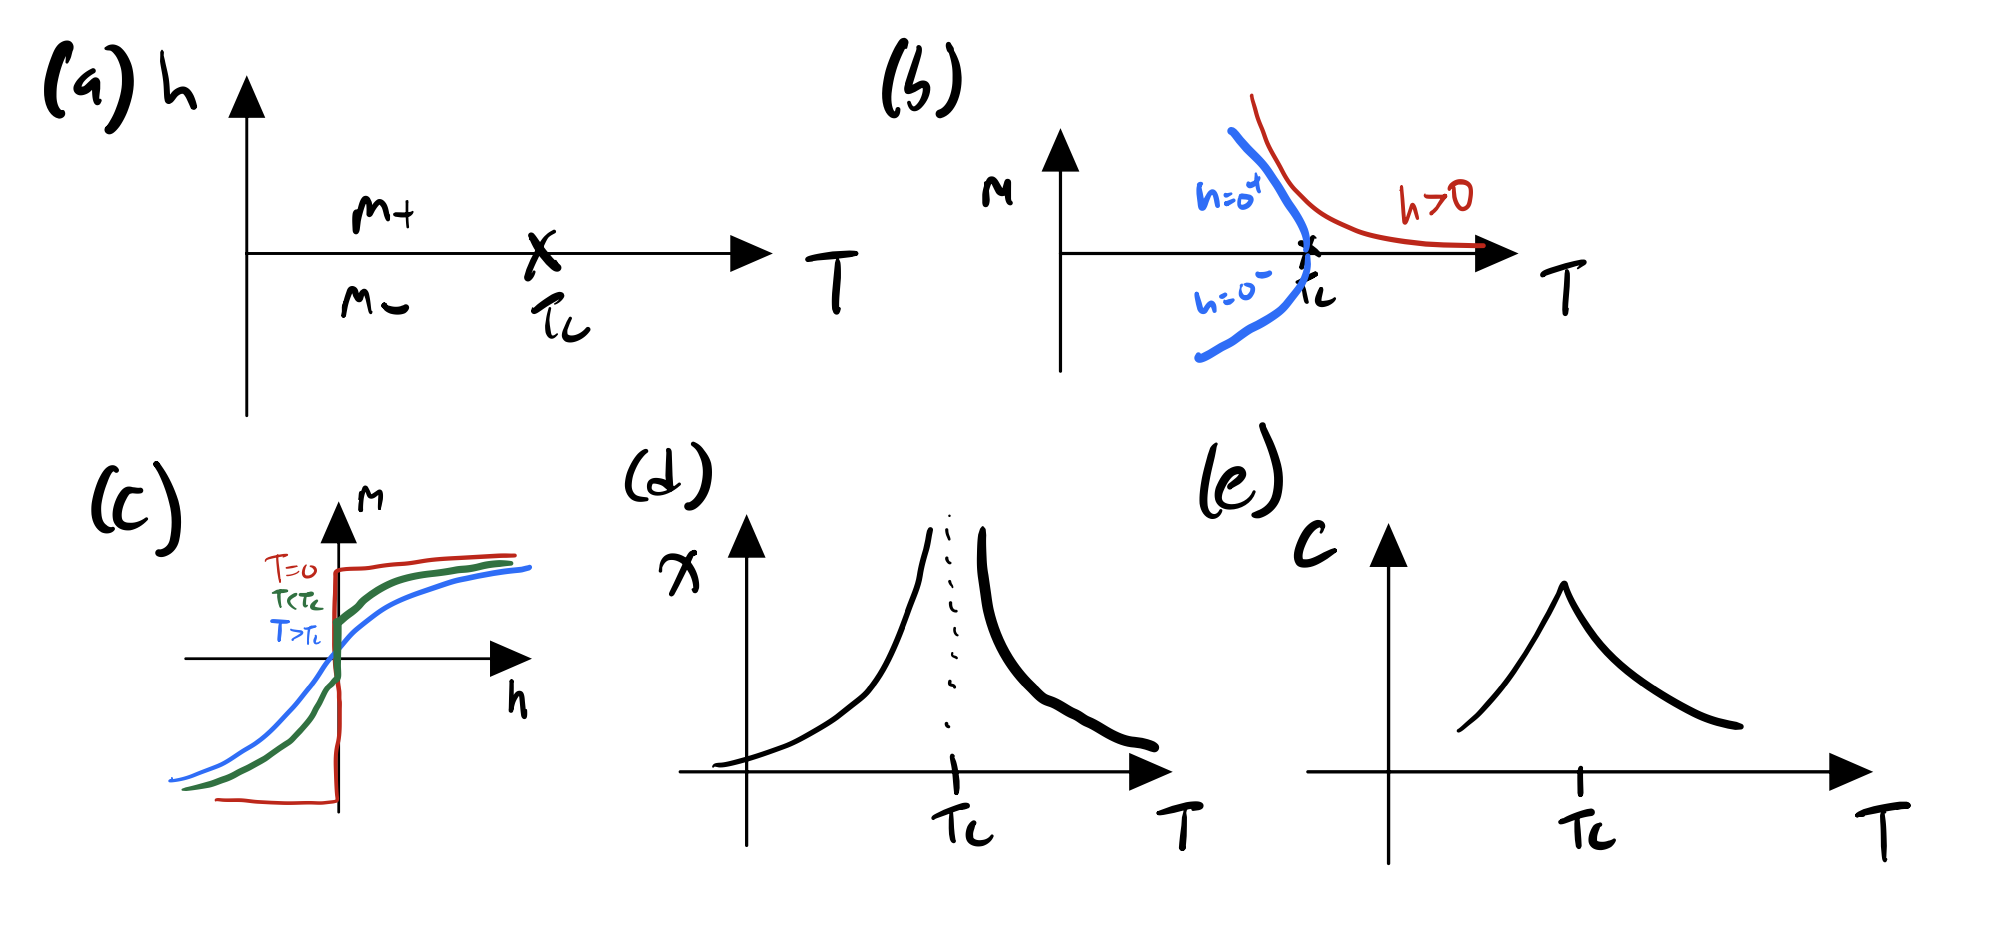
\includegraphics[scale=0.5]{Lectures/Figures/Various_plots.png}
    \caption{Plots of various measurable quantities and their behaviours near the critical temperature. (a) External field vs. Temperature. (b) Magnetization vs. Temperature for $h = 0$ and $h > 0$. (c) Magnetization vs. External field for various $T$. (d) Magnetic susceptibility vs. Temperature. (e) Heat capacity vs. Temperature.}
    \label{<label>}
\end{figure}

How do we calculate these quantities? We start with some partition function:
\begin{equation}
    Z = \Tr (e^{-\beta(H_0 + m.h.)})
\end{equation}
with $\beta = (k_B T)^{-1}$, $H_0 = -J\sum_{ij}S_iS_j$ and $m.h. = -h\sum_i S_i$ (the magnetization in field $h$). The trace here is a shorthand to say we compute the exponential for every possible configuration of spins, with the terms weighted by the energy (you could do this numerically, e.g. by doing a Monte Carlo simulation).

If I have a partition function, I can compute things! In particular, if I want to compute the (average) magnetization:
\begin{equation}
    \avg{M} = \dpd{\ln Z}{(\beta h)} = \frac{1}{Z}\Tr(Me^{-\beta(H_0 + m.h.)})
\end{equation}
We can then compute $\chi$:
\begin{equation}
    \chi = \dpd{M}{h} = \beta\left[\frac{1}{Z}\Tr\left(M^2e^{-\beta H}\right) - \frac{1}{Z^2}\left(\Tr(Me^{-\beta H})\right)^2\right]
\end{equation}
Of we look at this carefully, we see the first term is the expectation of $M^2$ and the second term is the square of the expectation value of $M$, i.e.:
\begin{equation}
    \chi = \beta\left(\avg{M^2} - \avg{M}^2\right).
\end{equation}
Thus, the susceptibility tells you about fluctuations from the average.

This $M$ we have written here is an average over all configurations and over all space. We may also be interested in an average just over space. To this end, we may consider that the macroscopic magnetization is just the integral over the course-grained position dependent magnetization $m(x)$:
\begin{equation}
    M = \int d^3r m(x)
\end{equation}
from which:
\begin{equation}
    \chi = \beta \int d^3r d^3r' \left(\avg{m(r)m(r')} - \avg{m(r)}\avg{m(r')}\right).
\end{equation}
Now, if $r, r'$ are closeby, we expect the magnetization to be correlated, and if they are not, it depends on the ordering of the state. To this end, let us define here a connected average of $C$:
\begin{equation}
    \avg{m(r)m(r')}_C = \avg{(m(r) - \avg{m(r)})(m(r') - \avg{m(r')})} = G(r-r') - m^2
\end{equation}
where $G$ is a (Green's) function that depends on the distance $r-r'$. With this, the integral for $\chi$ becomes:
\begin{equation}
    \chi = \frac{V}{k_B T}\int dr \avg{m(r)m(0)}_C.
\end{equation}
So, interestingly, the susceptibility tells us something about the correlation function of spins. Generically, I expect this to decay:
\begin{equation}
    G(r) \sim e^{-r/\xi}
\end{equation}
which introduces the idea of a correlation length $\xi$. As I approach the phase transition, far-away degrees of freedom become more and more correlated- from the divergence of $\chi$ at the phase transition, we can also conclude that the correlation length $\xi$ must also diverge. Thus, we hypothesize:
\begin{equation}
    \xi \sim \abs{t}^{-\nu}.
\end{equation}
Also, notice that this happens on \emph{both} sides of the transition.

\subsection{Ginzburg-Landau Theory}
Another way we can thing about the partition function:
\begin{equation}
    Z(T) = \Tr(e^{-\beta H}) = \int \mathcal{D}[m(r)] W(m(r))
\end{equation}
I.e. look at all spatial configurations $\mathcal{D}[m(r)]$ of the order parameter, for each of these compute the statistical weight $W$, and add them up. 

We can use the $W$ to define a Hamiltonian:
\begin{equation}
    \beta H[m(r)] = -\ln W[m(r)]
\end{equation}
we do this to avoid writing down a microscopic Hamiltonian. Then, $\beta H[m(r)]$ is a functional of $m$, so:
\begin{equation}
    \beta H[m(r)] = \int d^dr \phi[m(r), r] = \int d^d r \phi[m, \nabla m, \nabla^2m, h, \ldots]
\end{equation}
We assume that $\phi$ is an analytic function of all of these variables, and stop at some point because we would consider some terms to not be relevant.